\documentclass[12pt,a4paper,twoside]{article}
\input{166.dat}
\usepackage{gensymb}
\usepackage{amsthm}
\usepackage{float}
\usepackage{siunitx}
\usepackage{amssymb}
\usepackage{float}
\usepackage{enumerate}
\usepackage{listings}
\usepackage{mathtools}
\usepackage[none]{hyphenat}
\usepackage{physics}
\newcommand\ddfrac[2]{\frac{\displaystyle #1}{\displaystyle #2}}
%\renewcommand{\familydefault}{\sfdefault}
\usepackage{booktabs,tabularx}
\renewcommand{\tabularxcolumn}{m}
\usepackage{listings}
\PassOptionsToPackage{hyphens}{url}\usepackage{hyperref}
\usepackage{color, colortbl}
\definecolor{cyan}{rgb}{0.85,0.89,0.95}
\renewcommand{\familydefault}{\sfdefault}

\begin{document}

\begin{titlepage}
\begin{center}
\vspace*{\fill}

\Huge{ Live-Feed-over-LAN Camera Spectrometer (LoLAN-CaS) Documentation} \\

\qquad
\qquad

\normalsize{Members: \\ 
Andrea Rica Advincula \\
Creo Baylon \\
Kenneth Domingo \\
Rene Principe Jr. \\
Lou Josef Tan}

\vspace*{\fill}
\end{center}
\end{titlepage}

\setcounter{page}{1}

\section{Overview}\label{sec:overview}
\medskip
The Live-Feed-over-LAN Camera Spectrometer (LoLAN-CaS) is an implementation of a spectrometer which can use any Android-based phone camera. On the hardware end, the camera broadcasts through a local area network (LAN) using a pre-set IP address. On the software end, the feed can be retrieved, processed, and displayed in real-time through any Python interpreter on a device connected on the same network. The spectrometer program depends on the following Python libraries:

\begin{itemize}

\item Numpy
\item Matplotlib
\item Scipy
\item OpenCV
\item Peakutils
\item URLlib

\end{itemize}

The current features are as follows:

\begin{itemize}

\item Calibration information can be set within the program itself.
\item Live feed of camera and corresponding intensity profile of a selected line scan region can be displayed in real-time on a computer with the required dependencies installed.
\item Scale of relative intensity profile can be set by the initial camera exposure settings but is always normalized.

\end{itemize}

\section{Setup}\label{sec:setup}\medskip

A spectrometer is composed of an emission source, an optical system, and a detector. The emission source is a gas-discharge lamp; the detector is a cellular phone; and the optical system was constructed out of office supplies. 

The construction of the optical system is fairly straight forward. A dark chamber was constructed by folding the cardboard box into a $10 \times 15 \times 8$ cm rectangular prism. The dimensions used are dependent on the average size of a smartphone; to hold the phone, extensions were attached to the rectangular prism as shown in Fig. \ref{fig1}. A rectangular hole was cut on the rectangular prism on the side of the phone holder; the hole was strategically placed on the location where the camera is positioned to which the diffraction grating is attached. On the far right corner from the diffraction grating, a portion of the prism is cut for the placement of the slit (Fig. \ref{fig2}); the slit was constructed by cutting a $6 \times 10$ cm rectangular piece of folder and slicing through the center, whose width is kept constant at approximately 1 mm. 

\begin{figure}[h!]
	\centering
	\subfloat[Side view of the setup.]{\makebox[0.5\textwidth]{{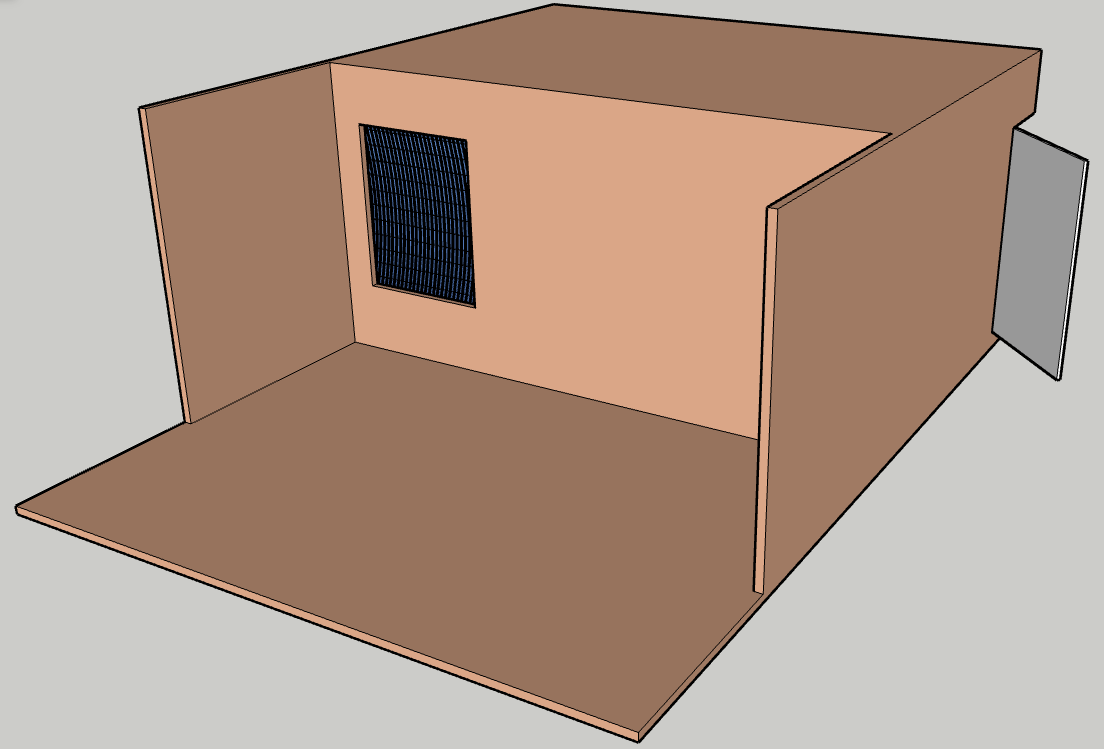
\includegraphics[width=0.4\textwidth]{setup.PNG}\label{fig1}}}}
	\subfloat[Tilted view of the setup.]{\makebox[0.5\textwidth]{{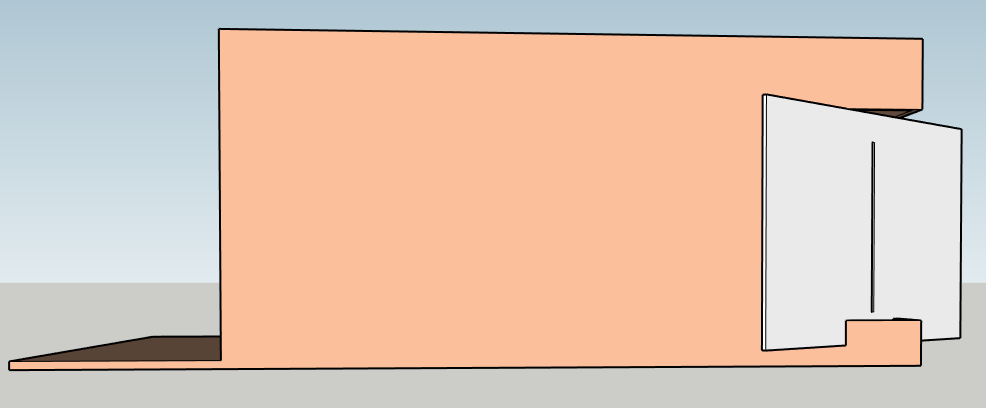
\includegraphics[width=0.48\textwidth]{right(1).PNG}\label{fig2}}}}
	\caption{3D design of LoLAN-CaS hardware using Sketchup}\label{figg1}
\end{figure}

\section{Operation}\label{sec:operation}\medskip
The optical system is positioned in front of the light source such that the slit is directly facing the light source; the slit width dictates the resolution of the entering light with enough intensity to be able to measure the spectral lines \cite{slit}. 

Since the diffraction grating used is a re-purposed CD, the gratings are radial which explains why the slit is positioned at an angle with respect to the grating. When the entering light strikes the diffraction grating, it splits into its spectral components which is then captured by the camera and displayed on the phone (Fig. \ref{setup}).

\begin{figure} [!h]
	\centering
	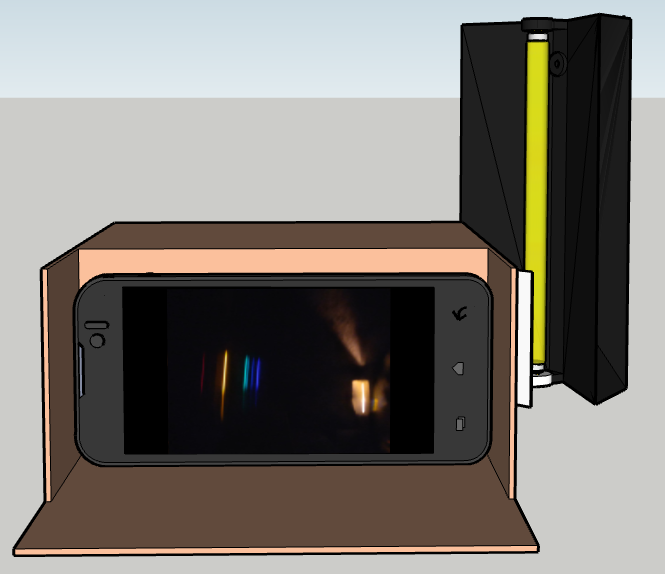
\includegraphics[width=0.6\linewidth]{setup1.PNG}
	\caption{\label{setup} Spectrometer schematic diagram}
\end{figure}

Using the Android app IPWebcam, the camera feed is broadcast in full resolution (1080p) through a local network. A computer or laptop connected on the same network can send an \texttt{HTTP GET} request to the phone's local IP and port to initiate the data stream. The image is then converted to grayscale and a pre-determined calibration curve is used to convert the pixel location values to wavelength.

\section{Program}\label{sec:program}\medskip

\subsection{\texttt{\footnotesize{Spectrometer}\normalsize{.\_\_init\_\_(calibrationLocation, calibrationWavelengths, lowerPix, upperPix, lowerBound, upperBound)}}}
Instantiates the \texttt{Spectrometer} object and takes the calibration arguments.

\begin{table}[H]
    \caption{Program initialization.}
    \begin{tabular}{>{\columncolor{cyan}}p{2in} p{4in}}
        \hline
        \textbf{Parameters} & \texttt{calibrationLocation : array\_like} \\
        &   Pixel locations of the peaks of the calibration image. \\ 
        & \texttt{calibrationWavelengths : array\_like} \\
        &   Corresponding wavelengths of \texttt{calibrationLocation}. \\
        & \texttt{lowerPix : int} \\
        &   Specifies pixel location of \texttt{lowerBound} (optional). \\
        & \texttt{upperPix : int} \\
        &   Specifies pixel location of \texttt{lowerBound} (optional). \\
        & \texttt{lowerBound : float} \\
        &	Specifies wavelength lower bound. \\
        & \texttt{upperBound : float} \\
        &	Specifies wavelength upper bound. \\ \hline
    \end{tabular}
    \label{tab:prog-init}
\end{table}

\subsection{\texttt{\footnotesize{Spectrometer}\normalsize{.plotCalibration()}}}

Plots the calibration curve and corresponding pixel-to-wavelength equation using linear regression.

\subsection{\texttt{\footnotesize{Spectrometer}\normalsize{.LineScan\_snapshot(image\_name, peaks, window\_length, polyorder)}}}

\begin{table}[H]
    \caption{\texttt{LineScan\_snapshot} arguments.}
    \begin{tabular}{>{\columncolor{cyan}}p{2in} p{4in}}
        \hline
        \textbf{Parameters} & \texttt{image\_name : str} \\
        &   File name of locally-stored image. \\ 
        & \texttt{peaks : bool} \\
        &   Sets whether peak points should be indicated on intensity profile. \\
        & \texttt{window\_length : int} \\
        &   Specifies window length of Savitsky-Golay filter. \\
        & \texttt{polyorder : int} \\
        &   Specifies polynomial order of Savitsky-Golay filter. \\ \hline
    \end{tabular}
    \label{tab:prog-lssnapshot}
\end{table}

\subsection{\texttt{\footnotesize{Spectrometer}\normalsize{.LineScan\_live(URL, show\_peaks, window\_length, polyorder)}}}

\begin{table}[H]
    \caption{\texttt{LineScan\_live} arguments.}
    \begin{tabular}{>{\columncolor{cyan}}p{2in} p{4in}}
        \hline
        \textbf{Parameters} & \texttt{URL : str} \\
        &   IP address of capturing device (Android-based phone camera only). \\ 
        & \texttt{show\_peaks : bool} \\
        &   Sets whether peak points should be indicated on intensity profile. \\
        & \texttt{window\_length : int} \\
        &   Specifies window length of Savitzky-Golay filter. \\
        & \texttt{polyorder : int} \\
        &   Specifies polynomial order of Savitzky-Golay filter. \\ \hline
    \end{tabular}
    \label{tab:prog-lslive}
\end{table}

\section{Demonstration}
Figure \ref{fig:calibration} shows the calibration curve obtained from a helium vapor lamp. An image is taken through the spectrometer setup and a line scan is taken through the apparent center of the spectral lines. Using literature values, each pixel is mapped to a wavelength using the equation $\textrm{wavelength} = 0.68(\textrm{pixel\_location}) - 855.76$, obtained by linear regression.

Figures \ref{fig:hydrogen}-\ref{fig:white} show the emission spectra of various light sources obtained using LoLAN-CaS. A snapshot of the camera feed is shown on the left-hand plot and its corresponding spectrum on the right-hand side. The portion taken from the line scan is shown as an inset on the right-hand figure. The wavelength values are also shown for each peak.

\begin{figure}[H]
	\centering
	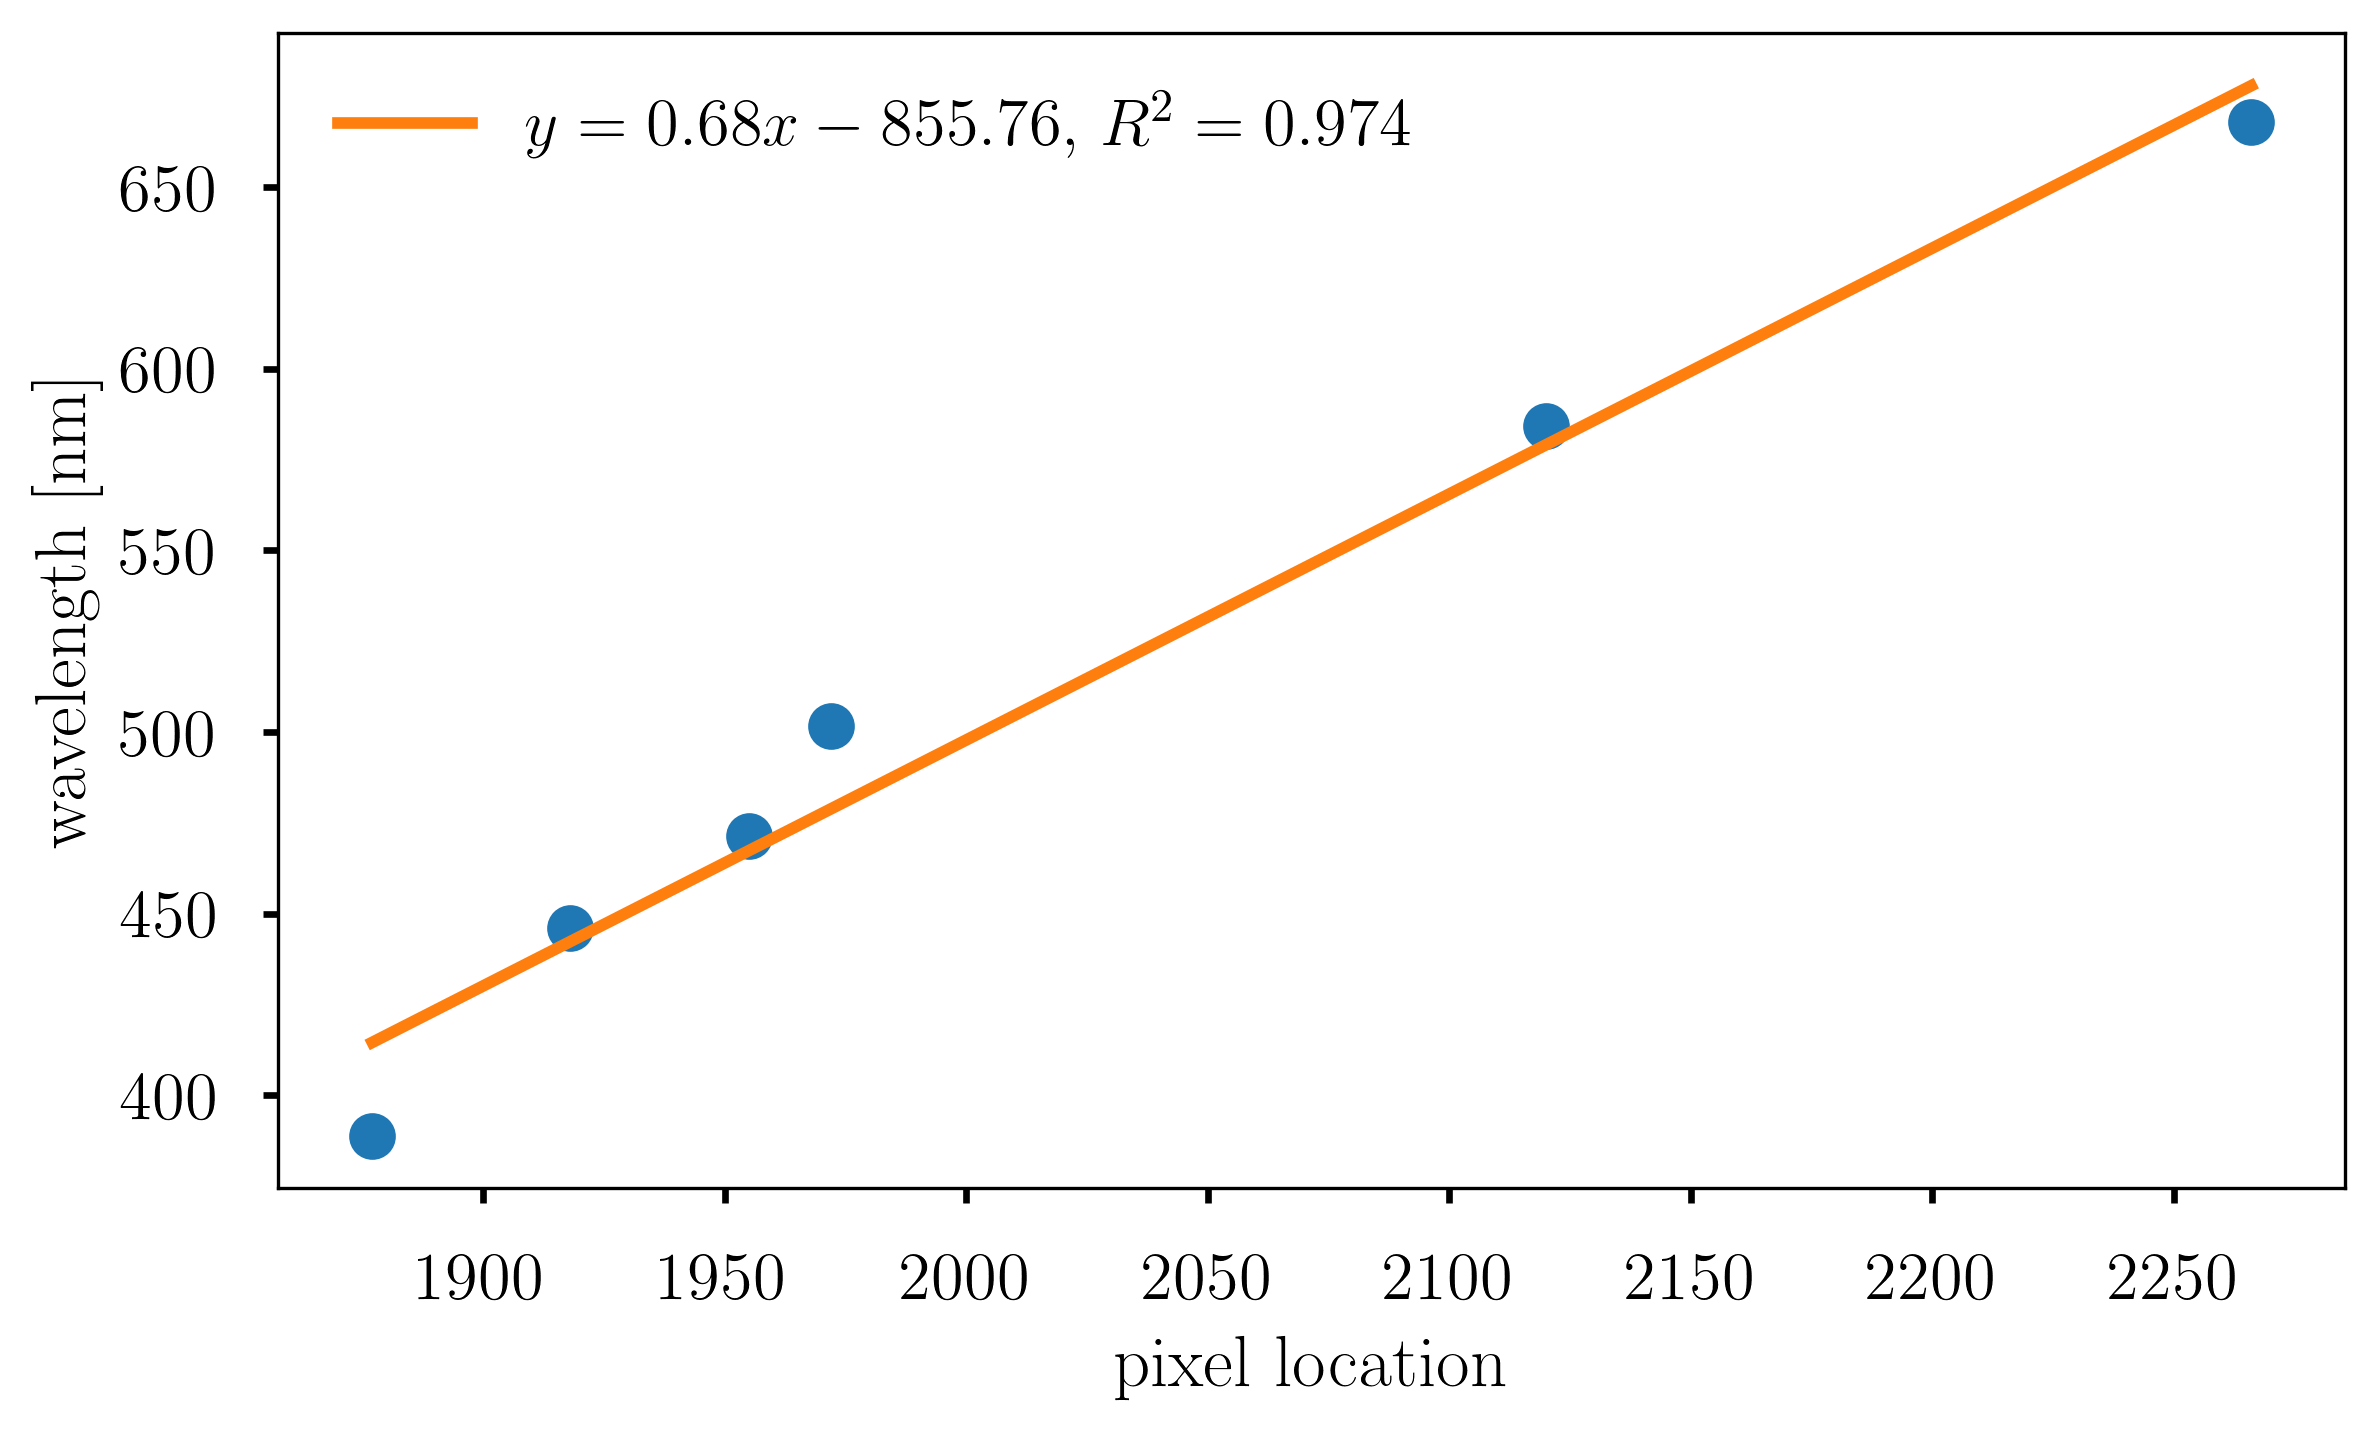
\includegraphics[width=0.9\linewidth]{calibcurve.png}
	\caption{Calibration curve obtained using a helium vapor lamp.}
	\label{fig:calibration}
\end{figure}

\begin{figure}[H]
	\centering
	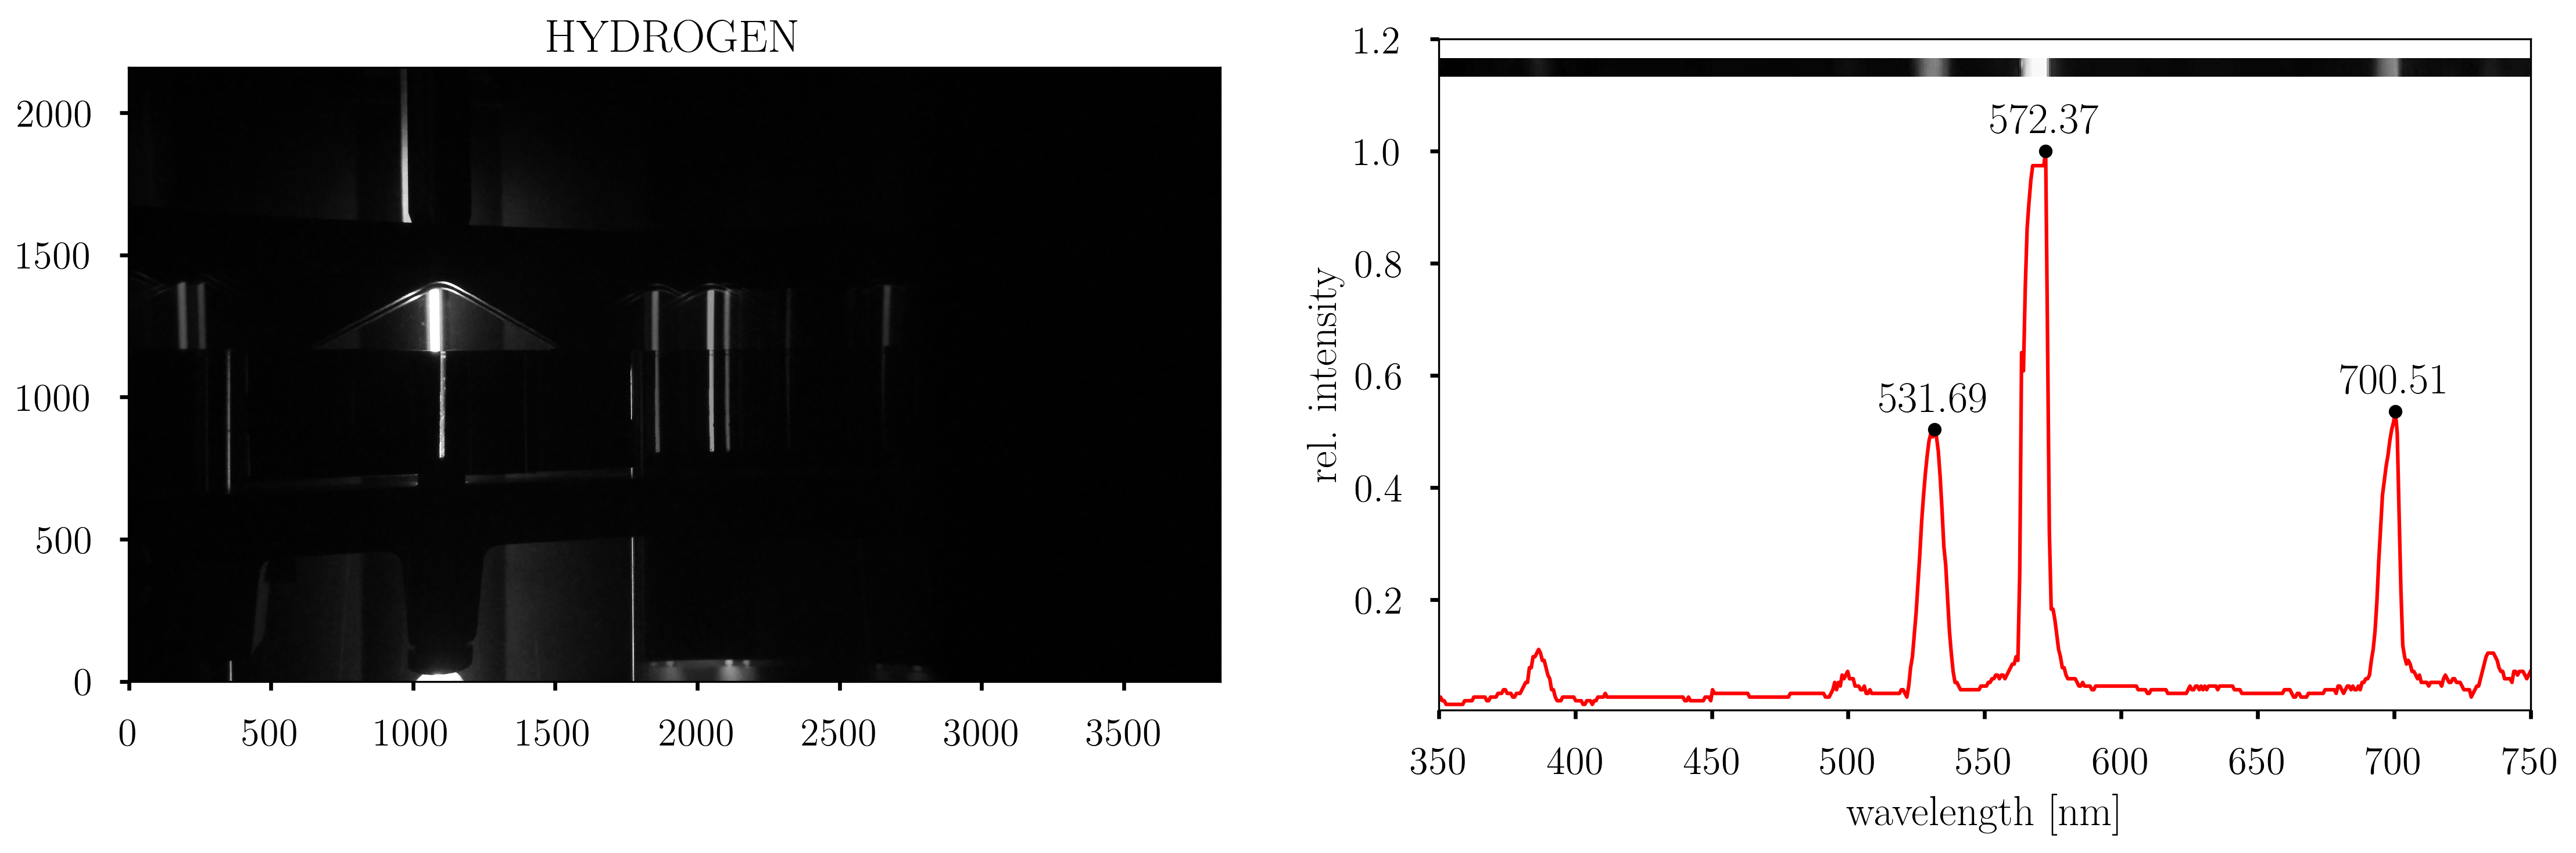
\includegraphics[width=\linewidth]{HYDROGEN.png}
	\caption{Emission spectrum of hydrogen.}
	\label{fig:hydrogen}
\end{figure}

\begin{figure}[H]
	\centering
	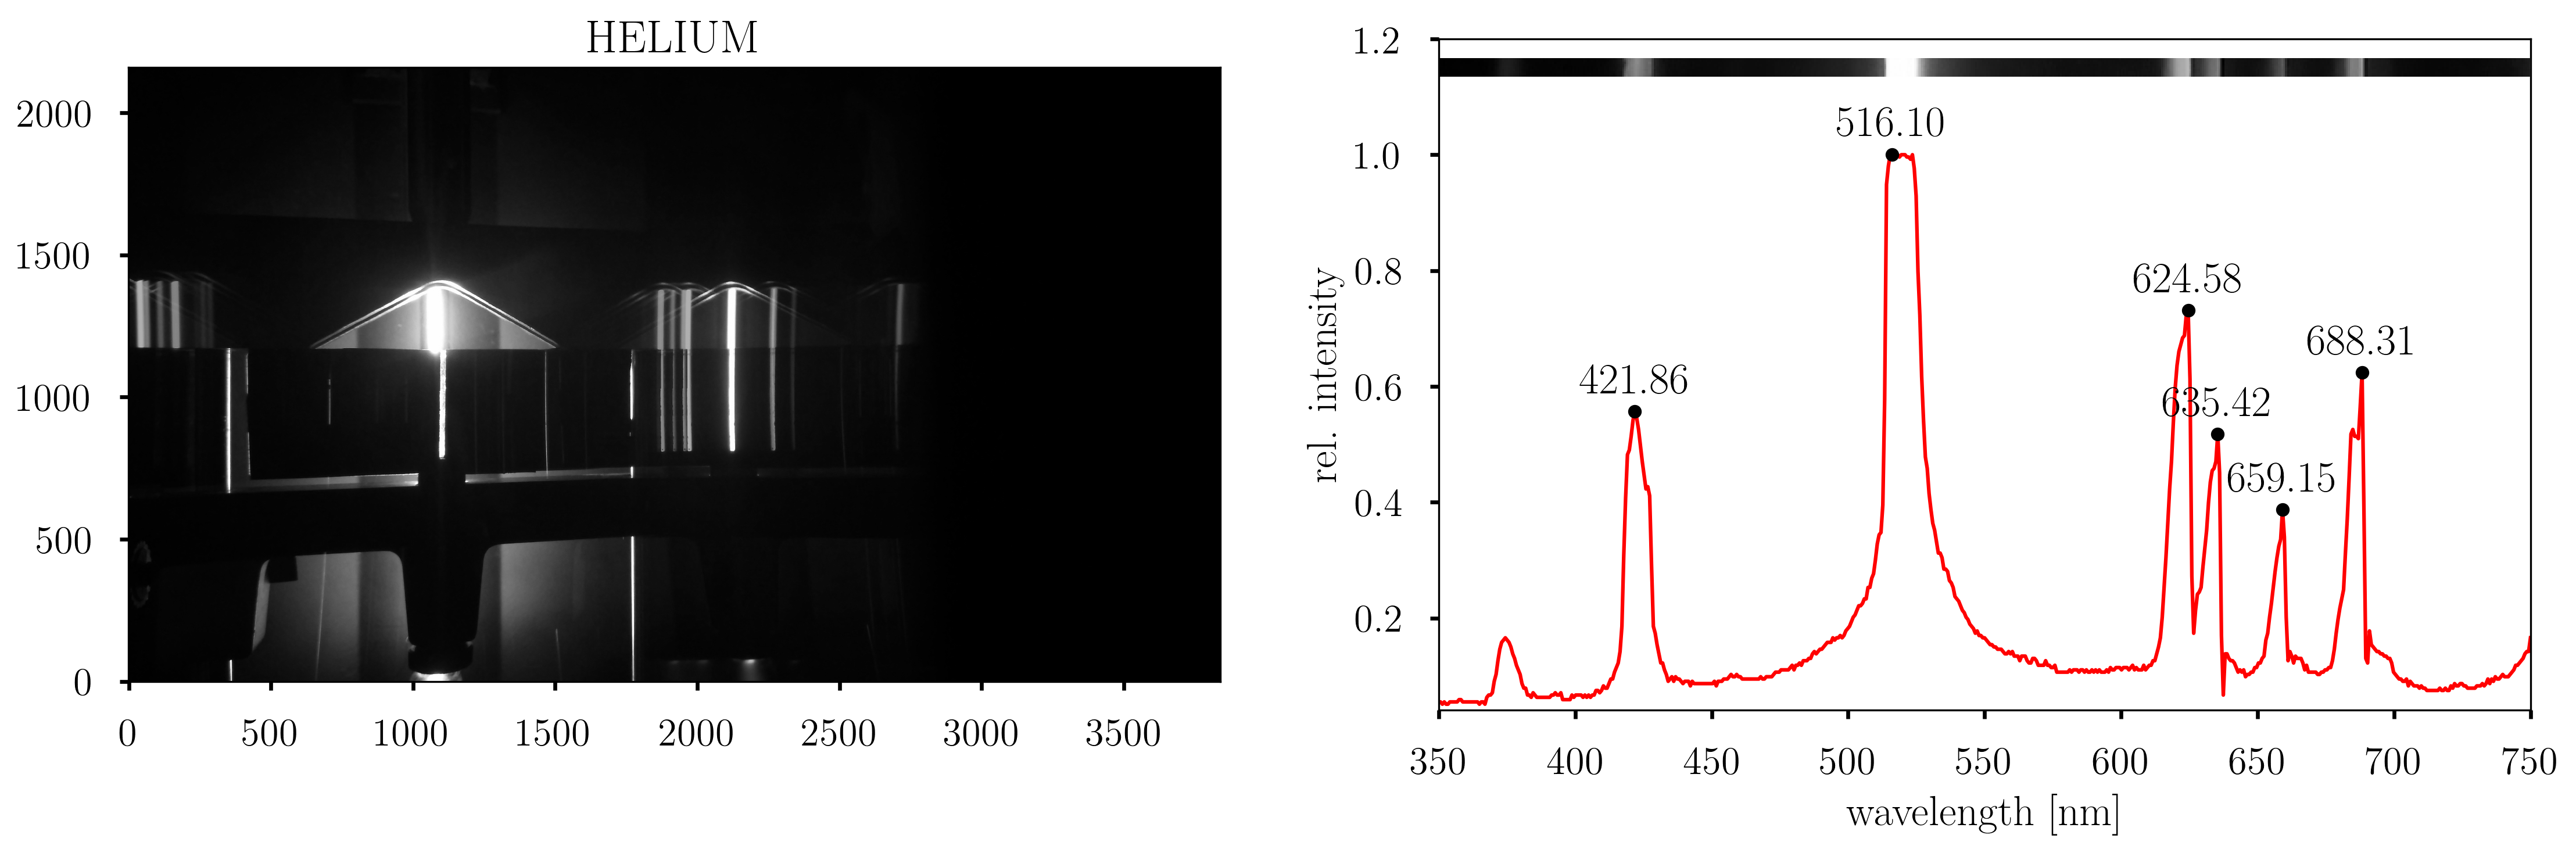
\includegraphics[width=\linewidth]{HELIUM.png}
	\caption{Emission spectrum of helium.}
	\label{fig:helium}
\end{figure}

\begin{figure}[H]
	\centering
	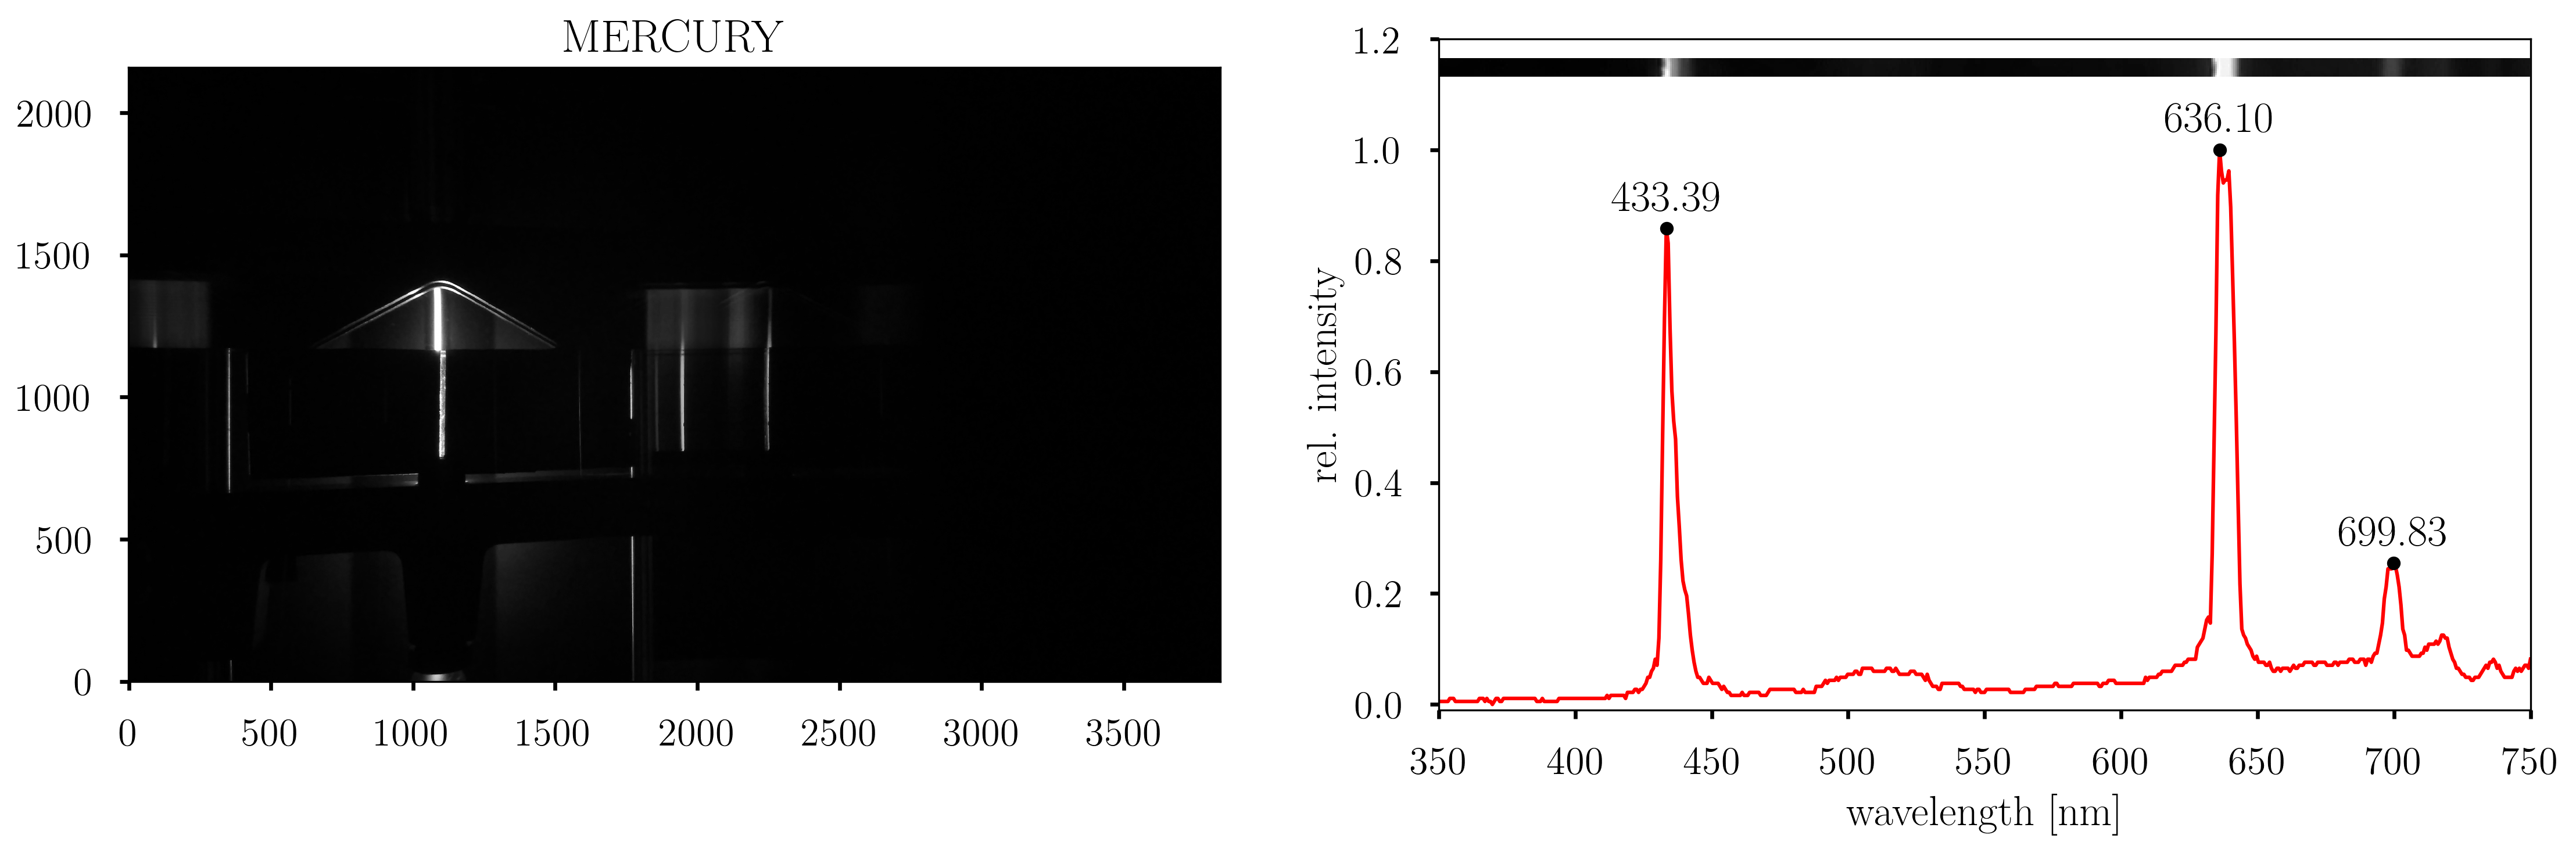
\includegraphics[width=\linewidth]{MERCURY.png}
	\caption{Emission spectrum of mercury.}
	\label{fig:mercury}
\end{figure}

\begin{figure}[H]
	\centering
	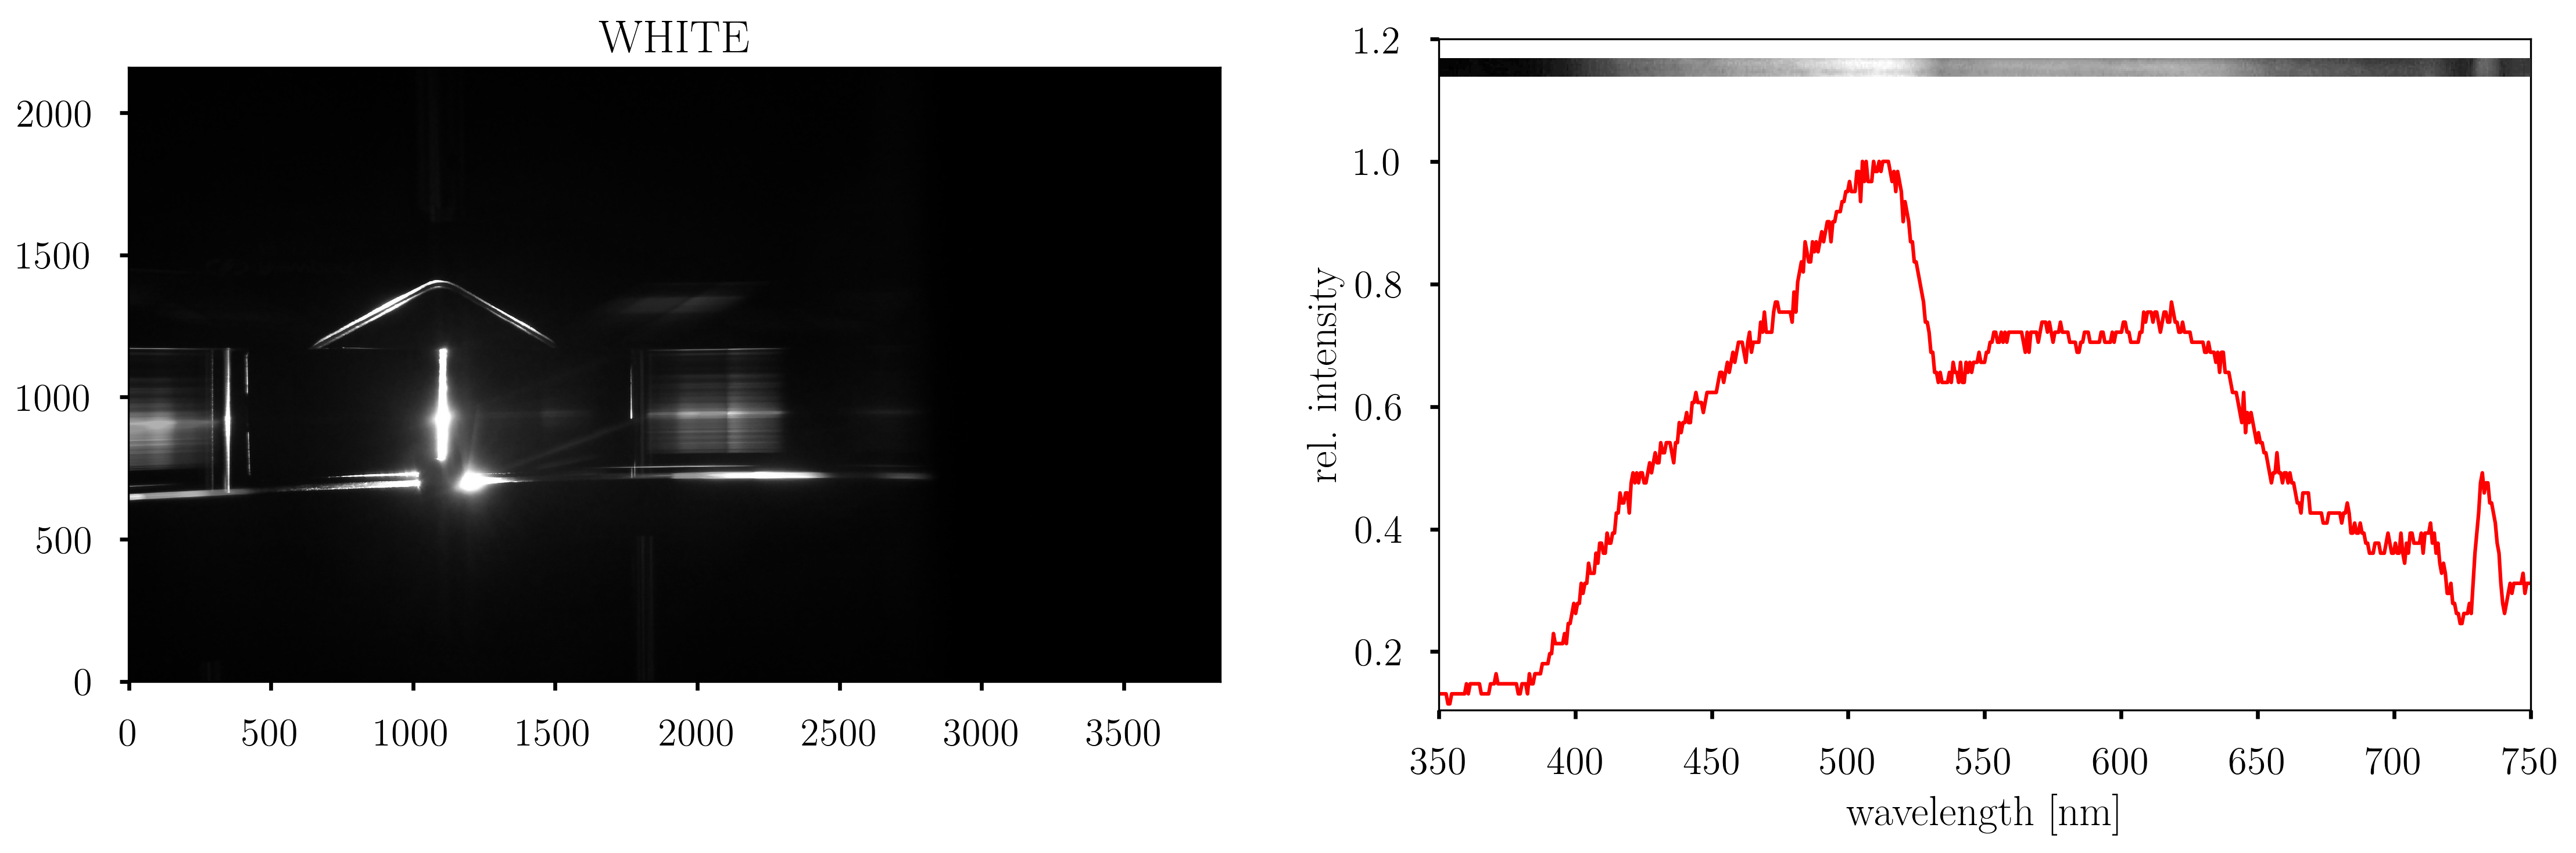
\includegraphics[width=\linewidth]{WHITE.png}
	\caption{Emission spectrum of a white LED flashlight.}
	\label{fig:white}
\end{figure}

\bibliographystyle{spp-bst}
\bibliography{bibfile}

\section*{Appendix}
Source code: \\
\url{https://colab.research.google.com/drive/1VMUdZ9GGeLgUW5F7rmk0VZNeu9xxkdcU}.

%\bibliographystyle{spp-bst}
%\bibliography{bibfile}

%\raggedbottom

%\pagebreak
%\pagebreak[3]
\iffalse
\newpage

\renewcommand\thefigure{A\arabic{figure}} 
\setcounter{figure}{0}
\fi %removing this will break the code for some reason

\end{document}

